\documentclass{article}
\usepackage{listings}
\usepackage{hyperref}
\usepackage{graphicx}

\author{Hendrik Schick, Tobias Dorra}
\title{Project for Deep learning in medical imaging: Segmentation - MIC \\ \begin{large} 
Task 2: Implementation I
\end{large}}

\begin{document}
	
	\maketitle

	\section{Task}

		The task was to implement the given model for image segmentation (nnUNet), train it with the given datasets and evaluate the performance.

	\section{Implementation}

		\subsection{Implemented Network architecture}

			Out of the tree possible training models ('2D U-Net', '3D U-Net', '3D U-Net Cascade'), we chose to use '3D U-Net' as a starting point. We made this choice, because choosing one of the 3d versions seemed to make sense based on the fact that we have 3d data. The cascade model is intended for the special case that the patch size chosen by nnUnet is relatively small compared to the overall size of the images and thus does not cover enough context. This did not seem to be the case with our datasets, so choosing the non-cascade 3d U-Net seemed to be the reasonable choice.

			The nnUNet makes only minor changes to the original U-Net, as it is described in the paper\footnote{U-Net: \url{https://arxiv.org/abs/1505.04597} - nnUNet: \url{https://arxiv.org/abs/1904.08128}}. Most notably:
			\begin{enumerate}
				\item Instead of 2d images, it uses 3d tensors. (obviously)
				\item Instead of ReLu, it uses LeakyReLu as activation function in the convolution layers.
				\item It uses padded convolutions, so that the convolution layers do not change the shape of the data.
				\item It does instance normalisation. (to be implemented)
			\end{enumerate}

			To obtain the exact (hyper)parameters to be used, we ran the 'Experiment Planning and Preprocessing' script from the nnUNet repository for both datasets. This analyzes the datasets and chooses suitable values for the patch size, convolution kernel sizes, number of pooling layers, etc.

			The parameters can be copied into our application and it will automatically build the corresponding model architecture with keras. To give an example, the resulting model architecture for the liver dataset can be seen in figure~\ref{fig:figure1}.

			\begin{figure}[htbp]
				\centering
				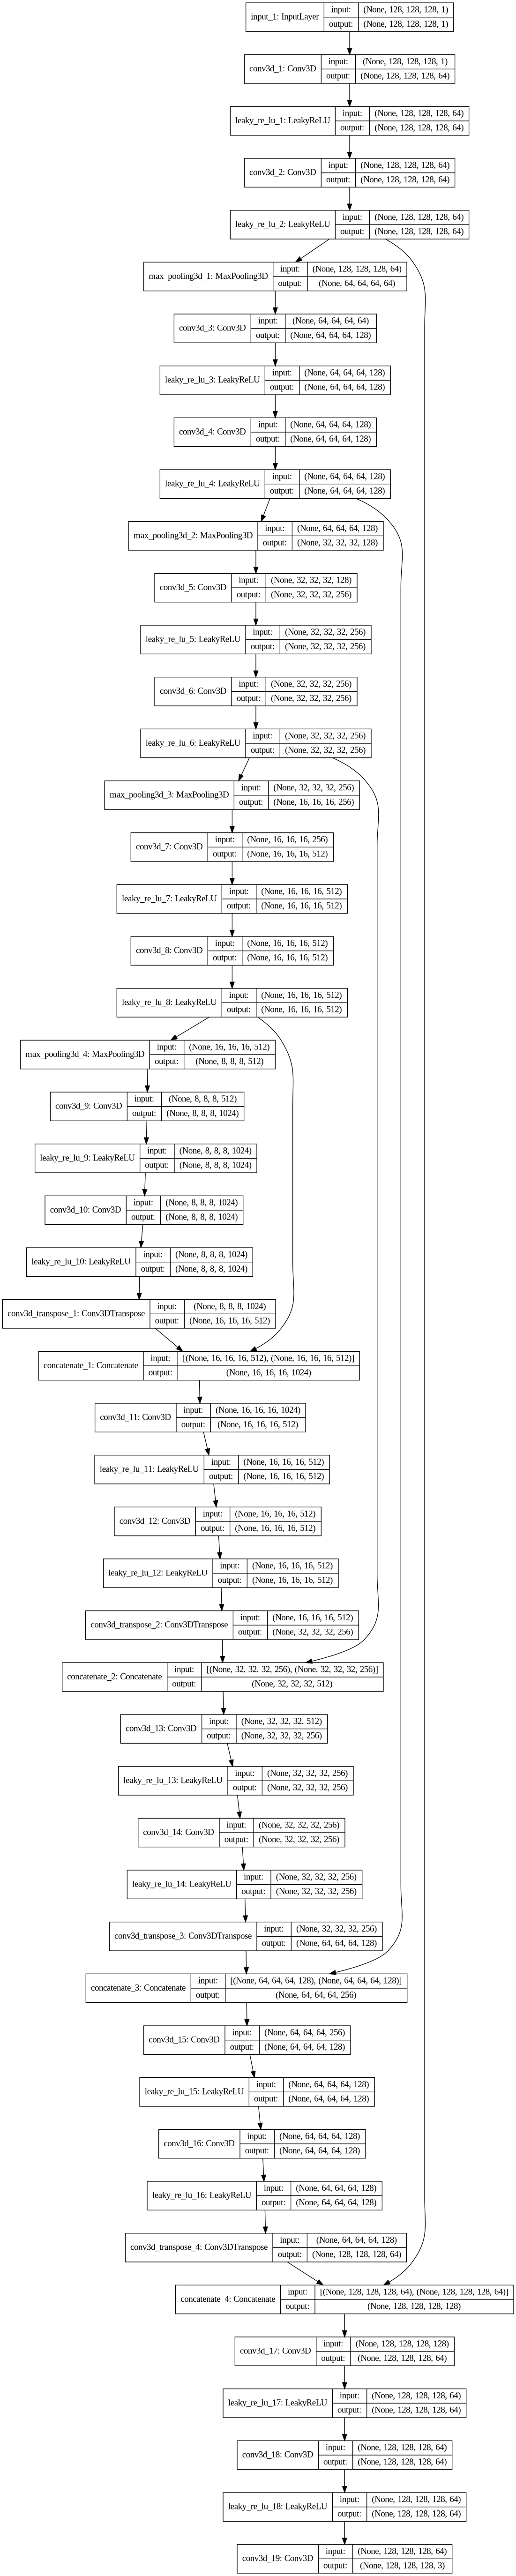
\includegraphics[height=\textheight]{model.png}
				\caption{Model architecture for the liver dataset.}
				\label{fig:figure1}
			\end{figure}

		\subsection{Preprocessing}

			We implemented the following preprocessing steps:

			\begin{enumerate}
			 	\item All images are rescaled, such that the real-world distance between two neighbouring voxels ('spacing') is always the same.
			 	\item Padding is added in case the patch size is larger than the image.
			 	\item Patches that match the size of the input layer are extracted from the image and used for training/testing.
			\end{enumerate} 

			The preprocessed images are cached on disk, so that it only has to be done once.

		\subsection{Training}

			The input files are split into a training and a testing set. The testing set consists of 10 randomly chosen images, the remaining images make up the training set.

			For training the model, the function train\_on\_batch from keras is used. This allows us to only keep a single batch in memory at a time, because the complete dataset is to large to store it in memory as a whole. The batch size is configurable.

			We are using the Adam optimizer with categorical crossentropy as loss function.

		\subsection{Evaluation}

			Results can be evaluated by calculating the intersection over union between the real segmentation and a predicted segmentation for each of the possible classes individually. This gives a value per class that is between $0$ and $1$, describing how well the individual classes overlap.

	\section{Problems and future tasks}

		Not for all of the metaparameters that were returned by the 'Experiment Planning and Preprocessing' script was it completely clear, what exactly they mean. This is, bacause the nnUNet source code is not very clean and the readme and paper don't go into enough detail. Most importently, the spacing information did not seem to match to what we saw in the training data - probably, because we did not interpret it correctly. As a result, we just hardcoded the target spacing in the resizing preprocessing step.

		We had enormous memory problems when testing on our personal machines. It was not possible, to run the network architecture as proposed by nnUNet on our private machines.

		We still need to run the training and evaluation on the GPU machines.

\end{document}
% LIVER_PATH + TRAINING + '/liver_3.nii.gz'
